\documentclass[11pt]{article}
\usepackage{fullpage,graphicx,float,amsmath,enumitem,hyperref}
\setlist{parsep=5.5pt}
\setlength{\parindent}{0pt}
\setlength{\parskip}{\baselineskip}

\usepackage{fancyhdr}
\pagestyle{fancy}
\lhead{Missing Data and LOD}
\rhead{Paul Harmon, Nnamdi Ezike, and Andrea Mack}
\setlength{\headheight}{18pt}
\setlength{\headsep}{2pt}

\title{Pea Lodging Final Report}
\author{Client: Jamin Smitchger\\
Consultants: Paul Harmon, Nnamdi Ezike, and Andrea Mack}
\date{December 16, 2016}

\begin{document}
\maketitle





\section{Introduction}
Jamin is a Ph.D. student in the Department of Plant Sciences and Plant Pathology at MSU. The primary focus is his research is to associate variation in genetic expression with variation in the expression of several phenotypic traits. Genotypic and pheynotypic data were collected on 257 varities of pea, from two locations (Bozeman and Mocassin), in YEARS. Phenotypic data includes percent lodging, tendril length, tendril node length, nodes at 1st flow, maximum number of nodes, germination, number of branches, plant height, plant length, average total yield, main stem diameter, tiller diameter, ``comp" tiller diameter, and maturation time, totaling 14 traits. Data from 609 genetic markers were collected. The end result of Jamin's research will include a quantitative trait loci (QTL) analysis which will inform him about which genetic markers variation in genetic marker expression associated with variation in phenotypic traits. Prior to the QTL analysis, understanding of the data and methods are necessary. The report includes:

\begin{itemize}

\item Evaluation of correlations in pheynotypic data

\item Analysis of combining data from the different sites and years

\item Exploration of the rate of missing data

\item Explanation of significance thresholds for QTL 

\item Suggestions for future work
\end{itemize}

\section{Correlation Plots}
Correlation describes the strength and direction of a linear association. Specifically, this analyis examines Pearson Correlations because the varibles are measured on a quantiative scale.  The strength of the linear association between variables is measured on a scale between -1 (a perfect negative association) and 1 (a perfect positive association). Correlation does not imply causal relationships. In examining, for instance, the relationship between lodging and stem width, the pearson correlation would only give information about the linear association between the two variables.  Indeed, even a strong association between the two variables cannot be interpreted that stem width causes lodging; rather, we would simply say that the two variables are associated with each other.  Since the phenotypes in each year at each site are considered seperate response values, we consider fitting correlation plots for each site/year combination. 

\subsection{Sites and Years Combined}

The correlation between pairwise explanatory variables of the phenotypic data were assessed using the a pairwise correlation matrix. We assessed the pairwise correlations across sites for pairs of explanatory variables which were measured within these sites at least in two different years.

The pairwise correlation matrix below shows that germination which was measured in Bozeman for all 3 years has weak correlation against all the variables measured. Also results from Bozeman shows that tendril length node of the plant was moderately to strongly correlated with the average length and tendril length of the plant with correlation coefficients of 0.61 and 0.48 respectively. The branch number and tiller diameter of the plant were also moderately correlated (r = 0.47). The maturity time of the plant was strongly and moderately correlated with the maximum nodes (r=0.65) and nodes of 1st flow (r=0.48). In addition, a correlation coefficient of 0.81 was observed for nodes 1st flow and maximum nodes of the plants.

In Moccasin, only four variables were observed to have been measured both in 2015 and 2016. Of these variables, the length and main stem diameter of the plants are moderately correlated (r=-0.55). Also, the main stem diameter and root diameter of the plants are moderately correlated (r=0.45).

\begin{knitrout}\footnotesize
\definecolor{shadecolor}{rgb}{1, 1, 1}\color{fgcolor}

{\centering 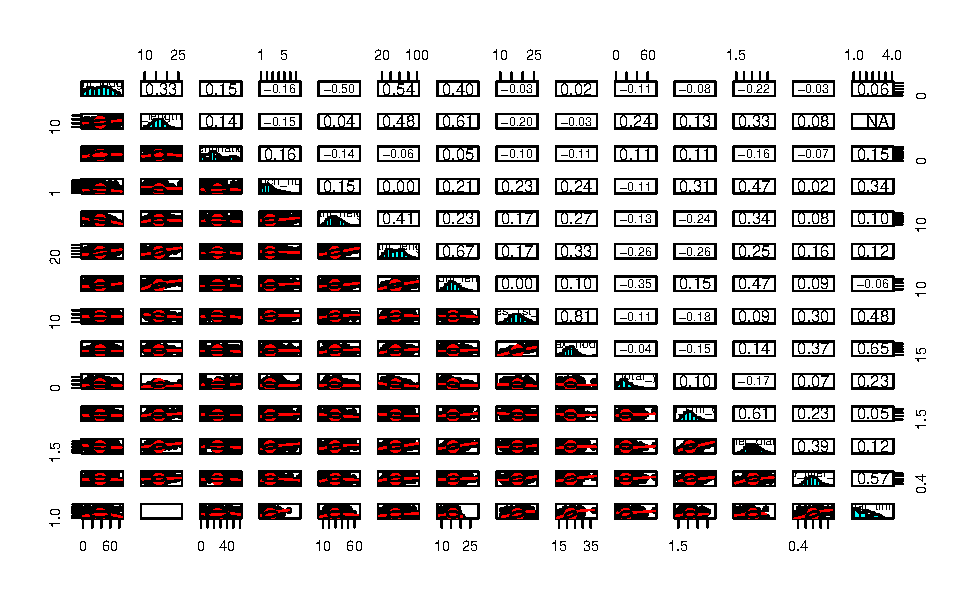
\includegraphics[width=\maxwidth]{figure/merged-1} 

}



\end{knitrout}

\subsection{Bozeman by Year}
We assessed the pairwise correlation of the different sites each year. In 2014, twelve pairs of explanatory variables had correlation coefficients between 0.42 and 0.91. The pairwise correlations are shown in the matrix below. Germination and total yield was strongly correlated (r=0.66) while the length and internode length of the plants recorded a very high correlation coefficient (r=0.91). In 2015 and 2016, of the pairwise combinations assessed, 28 combinations yielded correlation coefficients between 0.40 and 0.85. The results are presented in the pairwise correlation matrices below.

\begin{knitrout}\footnotesize
\definecolor{shadecolor}{rgb}{1, 1, 1}\color{fgcolor}\begin{kframe}


{\ttfamily\noindent\bfseries\color{errorcolor}{Error in eval(expr, envir, enclos): object 'bz16' not found}}

{\ttfamily\noindent\bfseries\color{errorcolor}{Error in colnames(bozeman16)[colnames(bozeman16) == "{}pctg\_Lodging\_boze\_2016"{}] <- "{}prcnt\_lodging"{}: object 'bozeman16' not found}}

{\ttfamily\noindent\bfseries\color{errorcolor}{Error in colnames(bozeman16)[colnames(bozeman16) == "{}GerminateNABozemanNA2016"{}] <- "{}germination"{}: object 'bozeman16' not found}}

{\ttfamily\noindent\bfseries\color{errorcolor}{Error in colnames(bozeman16)[colnames(bozeman16) == "{}Avg\_brnch\_numb\_boz\_2016"{}] <- "{}branch\_numb"{}: object 'bozeman16' not found}}

{\ttfamily\noindent\bfseries\color{errorcolor}{Error in colnames(bozeman16)[colnames(bozeman16) == "{}avg\_height\_boze\_2016"{}] <- "{}avg\_plant\_height"{}: object 'bozeman16' not found}}

{\ttfamily\noindent\bfseries\color{errorcolor}{Error in colnames(bozeman16)[colnames(bozeman16) == "{}avg\_length\_boze\_2016"{}] <- "{}avg\_plant\_length"{}: object 'bozeman16' not found}}

{\ttfamily\noindent\bfseries\color{errorcolor}{Error in colnames(bozeman16)[colnames(bozeman16) == "{}Mat\_time\_boze\_2016"{}] <- "{}maturity\_time"{}: object 'bozeman16' not found}}

{\ttfamily\noindent\bfseries\color{errorcolor}{Error in colnames(bozeman16)[colnames(bozeman16) == "{}avg\_tend\_length\_boze\_2016"{}] <- "{}tendril\_length"{}: object 'bozeman16' not found}}

{\ttfamily\noindent\bfseries\color{errorcolor}{Error in colnames(bozeman16)[colnames(bozeman16) == "{}Avg\_Main\_stem\_diam\_boze\_2016"{}] <- "{}main\_stem\_diam"{}: object 'bozeman16' not found}}

{\ttfamily\noindent\bfseries\color{errorcolor}{Error in colnames(bozeman16)[colnames(bozeman16) == "{}avg\_comp\_mn\_stm\_dia\_boze\_2016"{}] <- "{}comp\_main\_stem\_diam"{}: object 'bozeman16' not found}}

{\ttfamily\noindent\bfseries\color{errorcolor}{Error in colnames(bozeman16)[colnames(bozeman16) == "{}avg\_comp\_brnch\_diam\_boze\_2016"{}] <- "{}comp\_branch\_diam"{}: object 'bozeman16' not found}}

{\ttfamily\noindent\bfseries\color{errorcolor}{Error in colnames(bozeman16)[colnames(bozeman16) == "{}avg\_branch\_diam\_boze\_2016"{}] <- "{}branch\_diam"{}: object 'bozeman16' not found}}

{\ttfamily\noindent\bfseries\color{errorcolor}{Error in colnames(bozeman16)[colnames(bozeman16) == "{}comp\_brnch\_diam\_boze\_2016"{}] <- "{}comp\_branch\_diam"{}: object 'bozeman16' not found}}

{\ttfamily\noindent\bfseries\color{errorcolor}{Error in colnames(bozeman16)[colnames(bozeman16) == "{}avg\_root\_diam\_boze\_2016"{}] <- "{}root\_diam"{}: object 'bozeman16' not found}}

{\ttfamily\noindent\bfseries\color{errorcolor}{Error in ncol(x): object 'bozeman16' not found}}

{\ttfamily\noindent\bfseries\color{errorcolor}{Error in subset(bozeman16, select = -c(Line\_name, planting\_generation, : object 'bozeman16' not found}}

{\ttfamily\noindent\bfseries\color{errorcolor}{Error in eval(expr, envir, enclos): object 'bozeman16v2' not found}}

{\ttfamily\noindent\bfseries\color{errorcolor}{Error in ncol(x): object 'bozeman16v3' not found}}

{\ttfamily\noindent\bfseries\color{errorcolor}{Error in eval(expr, envir, enclos): object 'bz14' not found}}

{\ttfamily\noindent\bfseries\color{errorcolor}{Error in colnames(bozeman14)[colnames(bozeman14) == "{}Prcnt.Lodging"{}] <- "{}prcnt\_lodging"{}: object 'bozeman14' not found}}

{\ttfamily\noindent\bfseries\color{errorcolor}{Error in colnames(bozeman14)[colnames(bozeman14) == "{}Germination.2014.."{}] <- "{}gemination"{}: object 'bozeman14' not found}}

{\ttfamily\noindent\bfseries\color{errorcolor}{Error in colnames(bozeman14)[colnames(bozeman14) == "{}branch.numb.2014"{}] <- "{}branch\_numb"{}: object 'bozeman14' not found}}

{\ttfamily\noindent\bfseries\color{errorcolor}{Error in colnames(bozeman14)[colnames(bozeman14) == "{}height"{}] <- "{}plant\_height"{}: object 'bozeman14' not found}}

{\ttfamily\noindent\bfseries\color{errorcolor}{Error in colnames(bozeman14)[colnames(bozeman14) == "{}length"{}] <- "{}plant\_length"{}: object 'bozeman14' not found}}

{\ttfamily\noindent\bfseries\color{errorcolor}{Error in colnames(bozeman14)[colnames(bozeman14) == "{}tendril.length.14.node.2014"{}] <- "{}tendril\_length\_node"{}: object 'bozeman14' not found}}

{\ttfamily\noindent\bfseries\color{errorcolor}{Error in colnames(bozeman14)[colnames(bozeman14) == "{}tendril.length.2014"{}] <- "{}tendril\_length"{}: object 'bozeman14' not found}}

{\ttfamily\noindent\bfseries\color{errorcolor}{Error in colnames(bozeman14)[colnames(bozeman14) == "{}Nodes.1st.flow.2014"{}] <- "{}nodes\_1st\_flow"{}: object 'bozeman14' not found}}

{\ttfamily\noindent\bfseries\color{errorcolor}{Error in colnames(bozeman14)[colnames(bozeman14) == "{}max.nodes.2014"{}] <- "{}max\_nodes"{}: object 'bozeman14' not found}}

{\ttfamily\noindent\bfseries\color{errorcolor}{Error in colnames(bozeman14)[colnames(bozeman14) == "{}internode.length.2014"{}] <- "{}internode\_length"{}: object 'bozeman14' not found}}

{\ttfamily\noindent\bfseries\color{errorcolor}{Error in colnames(bozeman14)[colnames(bozeman14) == "{}Total.yield.2014"{}] <- "{}total\_yield"{}: object 'bozeman14' not found}}

{\ttfamily\noindent\bfseries\color{errorcolor}{Error in colnames(bozeman14)[colnames(bozeman14) == "{}Avg.Yld.Plant.2014"{}] <- "{}avg\_total\_yield"{}: object 'bozeman14' not found}}

{\ttfamily\noindent\bfseries\color{errorcolor}{Error in colnames(bozeman14)[colnames(bozeman14) == "{}Main.stm.diameter.2014"{}] <- "{}main\_stm\_diam"{}: object 'bozeman14' not found}}

{\ttfamily\noindent\bfseries\color{errorcolor}{Error in colnames(bozeman14)[colnames(bozeman14) == "{}Average.compressed.main.stem.thickness.2014"{}] <- "{}comp\_main\_stm"{}: object 'bozeman14' not found}}

{\ttfamily\noindent\bfseries\color{errorcolor}{Error in colnames(bozeman14)[colnames(bozeman14) == "{}Tiller.diameter.2014"{}] <- "{}tiller\_diam"{}: object 'bozeman14' not found}}

{\ttfamily\noindent\bfseries\color{errorcolor}{Error in colnames(bozeman14)[colnames(bozeman14) == "{}compressed.tiller.thickness.2014"{}] <- "{}comp\_tiller\_diam"{}: object 'bozeman14' not found}}

{\ttfamily\noindent\bfseries\color{errorcolor}{Error in colnames(bozeman14)[colnames(bozeman14) == "{}length.1"{}] <- "{}length\_1"{}: object 'bozeman14' not found}}

{\ttfamily\noindent\bfseries\color{errorcolor}{Error in subset(bozeman14, select = -c(DNA.GENERATION, LINE.., Germination.2014NACHECKED, : object 'bozeman14' not found}}

{\ttfamily\noindent\bfseries\color{errorcolor}{Error in eval(expr, envir, enclos): object 'bozeman14' not found}}

{\ttfamily\noindent\bfseries\color{errorcolor}{Error in ncol(x): object 'bozeman14' not found}}

{\ttfamily\noindent\bfseries\color{errorcolor}{Error in eval(expr, envir, enclos): object 'bz15' not found}}

{\ttfamily\noindent\bfseries\color{errorcolor}{Error in colnames(bozeman15)[colnames(bozeman15) == "{}Yield"{}] <- "{}yield"{}: object 'bozeman15' not found}}

{\ttfamily\noindent\bfseries\color{errorcolor}{Error in colnames(bozeman15)[colnames(bozeman15) == "{}X..GERMINATION.AVG.with.bad.germinating.lines.left.in.and.adjusted.for.seeds.planted"{}] <- "{}avg\_germination"{}: object 'bozeman15' not found}}

{\ttfamily\noindent\bfseries\color{errorcolor}{Error in colnames(bozeman15)[colnames(bozeman15) == "{}X..of.branch"{}] <- "{}branch\_numb"{}: object 'bozeman15' not found}}

{\ttfamily\noindent\bfseries\color{errorcolor}{Error in colnames(bozeman15)[colnames(bozeman15) == "{}plants.harvested"{}] <- "{}plants\_harvested"{}: object 'bozeman15' not found}}

{\ttfamily\noindent\bfseries\color{errorcolor}{Error in colnames(bozeman15)[colnames(bozeman15) == "{}X..Lodging"{}] <- "{}prcnt\_lodging"{}: object 'bozeman15' not found}}

{\ttfamily\noindent\bfseries\color{errorcolor}{Error in colnames(bozeman15)[colnames(bozeman15) == "{}Average.height"{}] <- "{}plant\_height"{}: object 'bozeman15' not found}}

{\ttfamily\noindent\bfseries\color{errorcolor}{Error in colnames(bozeman15)[colnames(bozeman15) == "{}average.length..Median.2015.40NA45cm."{}] <- "{}plant\_length"{}: object 'bozeman15' not found}}

{\ttfamily\noindent\bfseries\color{errorcolor}{Error in colnames(bozeman15)[colnames(bozeman15) == "{}Mat.time"{}] <- "{}maturity\_time"{}: object 'bozeman15' not found}}

{\ttfamily\noindent\bfseries\color{errorcolor}{Error in colnames(bozeman15)[colnames(bozeman15) == "{}tendril.width"{}] <- "{}tendril\_width"{}: object 'bozeman15' not found}}

{\ttfamily\noindent\bfseries\color{errorcolor}{Error in colnames(bozeman15)[colnames(bozeman15) == "{}tendril.Length"{}] <- "{}tendril\_length"{}: object 'bozeman15' not found}}

{\ttfamily\noindent\bfseries\color{errorcolor}{Error in colnames(bozeman15)[colnames(bozeman15) == "{}Nodes.1st.flow"{}] <- "{}nodes\_1st\_flow"{}: object 'bozeman15' not found}}

{\ttfamily\noindent\bfseries\color{errorcolor}{Error in colnames(bozeman15)[colnames(bozeman15) == "{}max.nodes"{}] <- "{}max\_nodes"{}: object 'bozeman15' not found}}

{\ttfamily\noindent\bfseries\color{errorcolor}{Error in colnames(bozeman15)[colnames(bozeman15) == "{}main.stem.DIAm.avg"{}] <- "{}main\_stem\_diam"{}: object 'bozeman15' not found}}

{\ttfamily\noindent\bfseries\color{errorcolor}{Error in colnames(bozeman15)[colnames(bozeman15) == "{}Main.stem.comp..avg"{}] <- "{}comp\_main\_stem\_diam"{}: object 'bozeman15' not found}}

{\ttfamily\noindent\bfseries\color{errorcolor}{Error in colnames(bozeman15)[colnames(bozeman15) == "{}tiller.Diam.AVG"{}] <- "{}tiller\_diam"{}: object 'bozeman15' not found}}

{\ttfamily\noindent\bfseries\color{errorcolor}{Error in colnames(bozeman15)[colnames(bozeman15) == "{}tiller.compressed.avg"{}] <- "{}comp\_tiller\_avg"{}: object 'bozeman15' not found}}

{\ttfamily\noindent\bfseries\color{errorcolor}{Error in colnames(bozeman15)[colnames(bozeman15) == "{}Root.compressed.avg"{}] <- "{}avg\_comp\_root"{}: object 'bozeman15' not found}}

{\ttfamily\noindent\bfseries\color{errorcolor}{Error in colnames(bozeman15)[colnames(bozeman15) == "{}avg.main..side.brnch.root"{}] <- "{}main\_branch\_root"{}: object 'bozeman15' not found}}

{\ttfamily\noindent\bfseries\color{errorcolor}{Error in subset(bozeman15, select = -c(line.., average.lodging.Moccasin.2015, : object 'bozeman15' not found}}

{\ttfamily\noindent\bfseries\color{errorcolor}{Error in eval(expr, envir, enclos): object 'bozeman15' not found}}

{\ttfamily\noindent\bfseries\color{errorcolor}{Error in ncol(x): object 'bozeman15' not found}}\end{kframe}
\end{knitrout}

\subsection{Moccasin by Year}

\begin{knitrout}\footnotesize
\definecolor{shadecolor}{rgb}{1, 1, 1}\color{fgcolor}\begin{kframe}


{\ttfamily\noindent\bfseries\color{errorcolor}{Error in eval(expr, envir, enclos): object 'moc16' not found}}

{\ttfamily\noindent\bfseries\color{errorcolor}{Error in colnames(moccasin16)[colnames(moccasin16) == "{}pctg\_Lodging\_boze\_2016"{}] <- "{}prcnt\_lodging"{}: object 'moccasin16' not found}}

{\ttfamily\noindent\bfseries\color{errorcolor}{Error in colnames(moccasin16)[colnames(moccasin16) == "{}X..GerminationNAMoccasinNA2016"{}] <- "{}prcnt\_germination"{}: object 'moccasin16' not found}}

{\ttfamily\noindent\bfseries\color{errorcolor}{Error in colnames(moccasin16)[colnames(moccasin16) == "{}Tendril.Length.2016"{}] <- "{}tendril\_length"{}: object 'moccasin16' not found}}

{\ttfamily\noindent\bfseries\color{errorcolor}{Error in colnames(moccasin16)[colnames(moccasin16) == "{}Avg.branch.number.2016"{}] <- "{}branch\_numb"{}: object 'moccasin16' not found}}

{\ttfamily\noindent\bfseries\color{errorcolor}{Error in colnames(moccasin16)[colnames(moccasin16) == "{}Mat.timeNA.MoccasinNA2016"{}] <- "{}maturity\_time"{}: object 'moccasin16' not found}}

{\ttfamily\noindent\bfseries\color{errorcolor}{Error in colnames(moccasin16)[colnames(moccasin16) == "{}AVG.length.moc.2016"{}] <- "{}plant\_length"{}: object 'moccasin16' not found}}

{\ttfamily\noindent\bfseries\color{errorcolor}{Error in colnames(moccasin16)[colnames(moccasin16) == "{}X.lodging.2016"{}] <- "{}prcnt\_lodging"{}: object 'moccasin16' not found}}

{\ttfamily\noindent\bfseries\color{errorcolor}{Error in colnames(moccasin16)[colnames(moccasin16) == "{}Main.stem.diam.avg.2016"{}] <- "{}main\_stem\_diam"{}: object 'moccasin16' not found}}

{\ttfamily\noindent\bfseries\color{errorcolor}{Error in colnames(moccasin16)[colnames(moccasin16) == "{}avg.branch.diam.2016"{}] <- "{}branch\_diam"{}: object 'moccasin16' not found}}

{\ttfamily\noindent\bfseries\color{errorcolor}{Error in colnames(moccasin16)[colnames(moccasin16) == "{}avg.root.diam.2016"{}] <- "{}root\_diam"{}: object 'moccasin16' not found}}

{\ttfamily\noindent\bfseries\color{errorcolor}{Error in subset(moccasin16, select = -c(Line.name, white.flow.moc.2016.checked, : object 'moccasin16' not found}}

{\ttfamily\noindent\bfseries\color{errorcolor}{Error in eval(expr, envir, enclos): object 'moccasin16' not found}}

{\ttfamily\noindent\bfseries\color{errorcolor}{Error in ncol(x): object 'moccasin16' not found}}

{\ttfamily\noindent\bfseries\color{errorcolor}{Error in eval(expr, envir, enclos): object 'moc15' not found}}

{\ttfamily\noindent\bfseries\color{errorcolor}{Error in colnames(moccasin15)[colnames(moccasin15) == "{}Lodging"{}] <- "{}prcnt\_lodging"{}: object 'moccasin15' not found}}

{\ttfamily\noindent\bfseries\color{errorcolor}{Error in colnames(moccasin15)[colnames(moccasin15) == "{}stress.minus.equation"{}] <- "{}stress\_m\_eqn"{}: object 'moccasin15' not found}}

{\ttfamily\noindent\bfseries\color{errorcolor}{Error in colnames(moccasin15)[colnames(moccasin15) == "{}original.stress.equation"{}] <- "{}ognl\_stress\_eqn"{}: object 'moccasin15' not found}}

{\ttfamily\noindent\bfseries\color{errorcolor}{Error in colnames(moccasin15)[colnames(moccasin15) == "{}stress.minus.equation.with.standard.thickness"{}] <- "{}SME\_Std\_thickn"{}: object 'moccasin15' not found}}

{\ttfamily\noindent\bfseries\color{errorcolor}{Error in colnames(moccasin15)[colnames(moccasin15) == "{}Height"{}] <- "{}plant\_height"{}: object 'moccasin15' not found}}

{\ttfamily\noindent\bfseries\color{errorcolor}{Error in colnames(moccasin15)[colnames(moccasin15) == "{}main.stem.DIAm.3"{}] <- "{}main\_stem\_diam"{}: object 'moccasin15' not found}}

{\ttfamily\noindent\bfseries\color{errorcolor}{Error in colnames(moccasin15)[colnames(moccasin15) == "{}tiller.Diam.3"{}] <- "{}tiller\_diam"{}: object 'moccasin15' not found}}

{\ttfamily\noindent\bfseries\color{errorcolor}{Error in colnames(moccasin15)[colnames(moccasin15) == "{}tiller.compressed.3"{}] <- "{}tiller\_comp"{}: object 'moccasin15' not found}}

{\ttfamily\noindent\bfseries\color{errorcolor}{Error in colnames(moccasin15)[colnames(moccasin15) == "{}till.comp.flex"{}] <- "{}till\_comp\_flex"{}: object 'moccasin15' not found}}

{\ttfamily\noindent\bfseries\color{errorcolor}{Error in colnames(moccasin15)[colnames(moccasin15) == "{}Flex.after.crushing"{}] <- "{}flex\_crush"{}: object 'moccasin15' not found}}

{\ttfamily\noindent\bfseries\color{errorcolor}{Error in colnames(moccasin15)[colnames(moccasin15) == "{}Root"{}] <- "{}root"{}: object 'moccasin15' not found}}

{\ttfamily\noindent\bfseries\color{errorcolor}{Error in subset(moccasin15, select = -c(X)): object 'moccasin15' not found}}

{\ttfamily\noindent\bfseries\color{errorcolor}{Error in ncol(x): object 'moccasin15' not found}}

{\ttfamily\noindent\bfseries\color{errorcolor}{Error in setwd("{}C:/Users/Paul/Documents"{}): cannot change working directory}}

{\ttfamily\noindent\bfseries\color{errorcolor}{Error in ncol(x): object 'moccasin16' not found}}\end{kframe}
\end{knitrout}


\section{Site Year Combinations for Lodging}


\begin{knitrout}\footnotesize
\definecolor{shadecolor}{rgb}{1, 1, 1}\color{fgcolor}\begin{kframe}


{\ttfamily\noindent\bfseries\color{errorcolor}{Error in setwd("{}C:/Users/Paul/Documents"{}): cannot change working directory}}\end{kframe}
\end{knitrout}

\subsection{Exploratory Analysis} 
The data were collected over a period of 4 field seasons at sites in Bozeman and 2 field seasons in Moccasin. Phenotypic data were analyzed in order to determine whether conditions were similar enough at each year/site combination to consider as a single dataset, or if they differ by enough that the sites and years need to be considered as different groups.  
Because lodging is considered the response of interest, we examine the Percent Lodging measured at each site/year combination. Note that Percent Lodging is not measured in the 2013 Bozeman data; we did not include it in this analysis. Given the result of the analysis, we do not need to consider it into the analysis to determine that there are differences in the year/site combinations.  Visually, we can plot the mean percent lodging at each year/site combination to get an idea of differences between the years and sites. Below, we have percent lodging at each site. It appears that the Moccasin sites tend to be slightly less variable; moreover, the median percent lodging at each site appeared to be higher in 2015 than in 2016.

\begin{knitrout}\footnotesize
\definecolor{shadecolor}{rgb}{1, 1, 1}\color{fgcolor}\begin{kframe}


{\ttfamily\noindent\bfseries\color{errorcolor}{Error in var(bz16\$X..Lodging.boze.2016, na.rm = TRUE): 'x' is NULL}}

{\ttfamily\noindent\bfseries\color{errorcolor}{Error in model.frame.default(formula = lodging \textasciitilde{} siteyear): variable lengths differ (found for 'siteyear')}}\end{kframe}
\end{knitrout}


\subsection{Interaction Plot}
If the sites are reasonably similar, we would expect to see parallel lines that are either overlapping or very near each other.  The red line for Bozeman indicates that average percent lodging was higher in Bozeman than in Moccasin in both 2015 and 2016; however it may also have been more variable than in Moccasin. While the blue line and red line are both decreasing from 2015 to 2016, the difference in slopes indicates that there may be some interaction between year/site combinations.  More formal testing is necessary to assess differences between year and site combinations, but this visualization indicates some evidence of a difference in lodging in each location and year.



\subsection{Regression Model}
  The regression treats Bozeman 2014 as the baseline (intercept) group. Each site-year combination is tested against the   baseline; small p-values indicate that the given group differs from the baseline. The p-values for each of the other site-year combinations are all quite small – the largest, for Bozeman 2015, is only 0.015, indicating strong evidence that each of the site/year combinations differ from the baseline. Moreover, the effect size ranges from 4 to 7 points on the 1-100 percent scale on which Percent Lodging is measured.  The confidence intervals given give estimates of the true mean lodging at each site/year combination. If all the intervals overlapped, we might have evidence that the combinations are at least reasonably similar; however, the 2016 interval in Moccasin and the 2014/2015 Bozeman intervals do not overlap. 





























